\documentclass{standalone}
\usepackage{tikz}
\usetikzlibrary{patterns, positioning}


\begin{document}
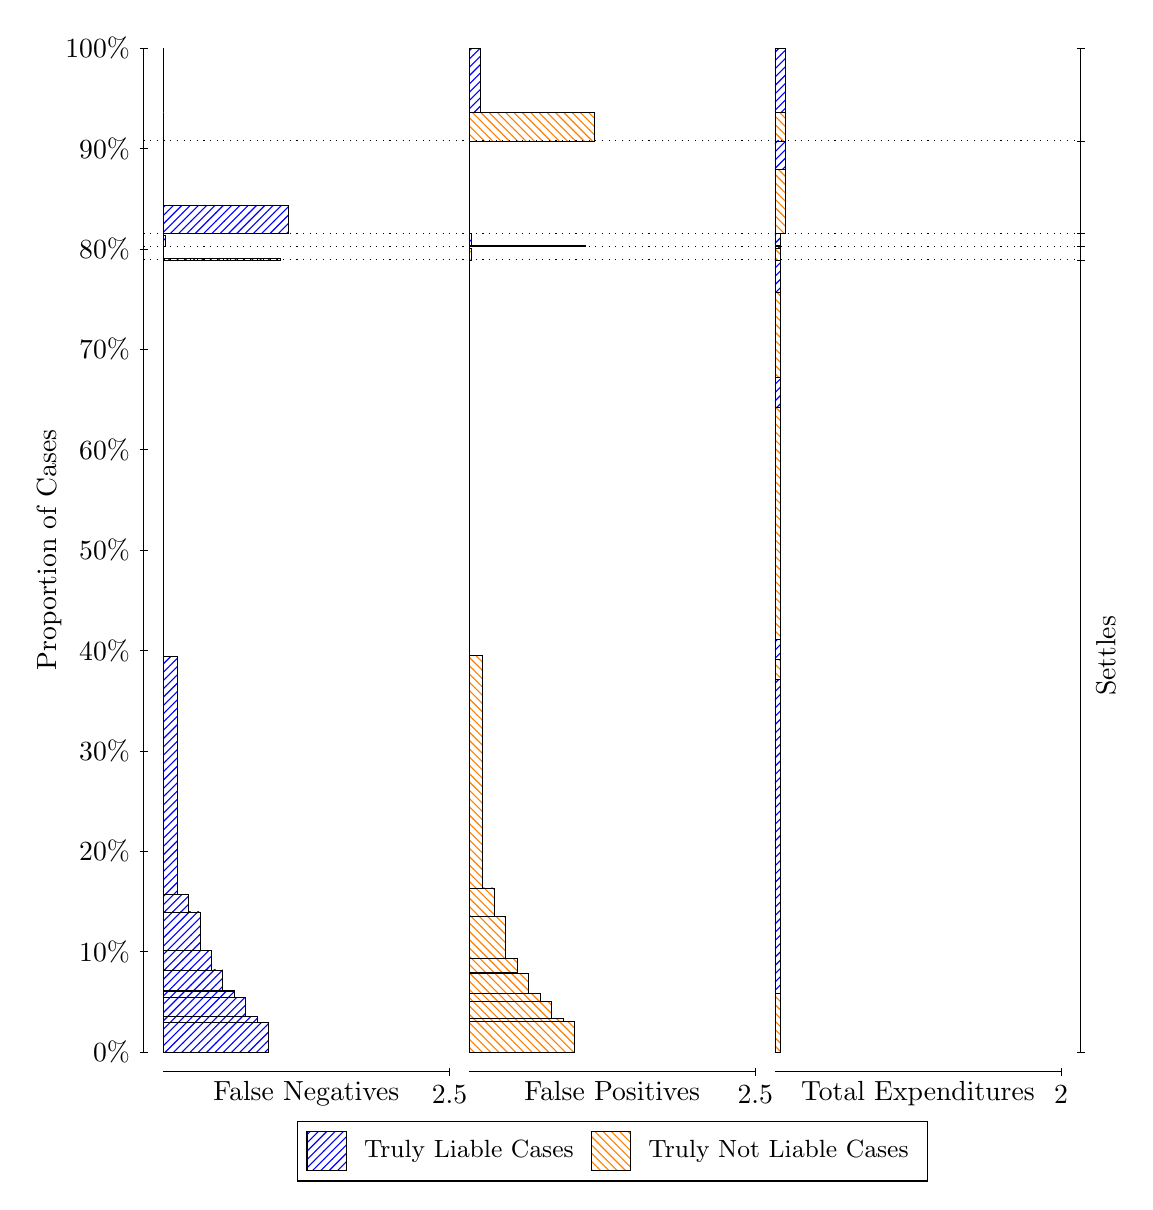
\begin{tikzpicture}
\draw[black, very thin] (1.5,1.75) -- (1.5,14.5);
\node[rotate=90, text=black, anchor=center] at (0.3, 8.125) {Proportion of Cases};
\draw[black, very thin] (1.45,1.75) -- (1.55,1.75);
\node[text=black, anchor=east] at (1.45, 1.75) {0\%};
\draw[black, very thin] (1.45,3.025) -- (1.55,3.025);
\node[text=black, anchor=east] at (1.45, 3.025) {10\%};
\draw[black, very thin] (1.45,4.3) -- (1.55,4.3);
\node[text=black, anchor=east] at (1.45, 4.3) {20\%};
\draw[black, very thin] (1.45,5.575) -- (1.55,5.575);
\node[text=black, anchor=east] at (1.45, 5.575) {30\%};
\draw[black, very thin] (1.45,6.85) -- (1.55,6.85);
\node[text=black, anchor=east] at (1.45, 6.85) {40\%};
\draw[black, very thin] (1.45,8.125) -- (1.55,8.125);
\node[text=black, anchor=east] at (1.45, 8.125) {50\%};
\draw[black, very thin] (1.45,9.4) -- (1.55,9.4);
\node[text=black, anchor=east] at (1.45, 9.4) {60\%};
\draw[black, very thin] (1.45,10.675) -- (1.55,10.675);
\node[text=black, anchor=east] at (1.45, 10.675) {70\%};
\draw[black, very thin] (1.45,11.95) -- (1.55,11.95);
\node[text=black, anchor=east] at (1.45, 11.95) {80\%};
\draw[black, very thin] (1.45,13.225) -- (1.55,13.225);
\node[text=black, anchor=east] at (1.45, 13.225) {90\%};
\draw[black, very thin] (1.45,14.5) -- (1.55,14.5);
\node[text=black, anchor=east] at (1.45, 14.5) {100\%};

\draw[black, very thin] (13.4,1.75) -- (13.4,14.5);
\draw[black, very thin] (13.35,1.75) -- (13.45,1.75);
\node[anchor=west] at (13.35, 1.75) {};
\draw[black, very thin] (13.35,11.81) -- (13.45,11.81);
\node[anchor=west] at (13.35, 11.81) {};
\draw[black, very thin] (13.35,11.977) -- (13.45,11.977);
\node[anchor=west] at (13.35, 11.977) {};
\draw[black, very thin] (13.35,12.144) -- (13.45,12.144);
\node[anchor=west] at (13.35, 12.144) {};
\draw[black, very thin] (13.35,13.32) -- (13.45,13.32);
\node[anchor=west] at (13.35, 13.32) {};
\draw[black, very thin] (13.35,14.5) -- (13.45,14.5);
\node[anchor=west] at (13.35, 14.5) {};

\draw[black, very thin, pattern color=blue, pattern=north east lines] (1.75,1.75) rectangle (3.0852,2.121);
\draw[black, very thin, pattern color=blue, pattern=north east lines] (1.75,2.121) rectangle (2.9399,2.1973);
\draw[black, very thin, pattern color=blue, pattern=north east lines] (1.75,2.1973) rectangle (2.7946,2.4426);
\draw[black, very thin, pattern color=blue, pattern=north east lines] (1.75,2.4426) rectangle (2.6492,2.5192);
\draw[black, very thin, pattern color=blue, pattern=north east lines] (1.75,2.5192) rectangle (2.6492,2.5343);
\draw[black, very thin, pattern color=blue, pattern=north east lines] (1.75,2.5343) rectangle (2.5039,2.7914);
\draw[black, very thin, pattern color=blue, pattern=north east lines] (1.75,2.7914) rectangle (2.3586,3.0406);
\draw[black, very thin, pattern color=blue, pattern=north east lines] (1.75,3.0406) rectangle (2.2133,3.5279);
\draw[black, very thin, pattern color=blue, pattern=north east lines] (1.75,3.5279) rectangle (2.0679,3.7476);
\draw[black, very thin, pattern color=blue, pattern=north east lines] (1.75,3.7476) rectangle (1.9226,6.7773);
\draw[black, very thin, pattern color=orange, pattern=north west lines] (1.75,6.7773) rectangle (1.75,11.81);
\draw[black, very thin, pattern color=blue, pattern=north east lines] (1.75,11.81) rectangle (3.2306,11.828);
\draw[black, very thin, pattern color=orange, pattern=north west lines] (1.75,11.828) rectangle (1.75,11.977);
\draw[black, very thin, pattern color=blue, pattern=north east lines] (1.75,11.977) rectangle (1.7773,12.126);
\draw[black, very thin, pattern color=orange, pattern=north west lines] (1.75,12.126) rectangle (1.75,12.144);
\draw[black, very thin, pattern color=blue, pattern=north east lines] (1.75,12.144) rectangle (3.3396,12.503);
\draw[black, very thin, pattern color=orange, pattern=north west lines] (1.75,12.503) rectangle (1.75,13.32);
\draw[black, very thin, pattern color=orange, pattern=north west lines] (1.75,13.32) rectangle (1.75,13.679);
\draw[black, very thin, pattern color=blue, pattern=north east lines] (1.75,13.679) rectangle (1.75,14.5);
\draw[black, very thin, pattern color=orange, pattern=north west lines] (5.6333,1.75) rectangle (6.9686,2.1375);
\draw[black, very thin, pattern color=orange, pattern=north west lines] (5.6333,2.1375) rectangle (6.8233,2.1745);
\draw[black, very thin, pattern color=orange, pattern=north west lines] (5.6333,2.1745) rectangle (6.6779,2.3899);
\draw[black, very thin, pattern color=orange, pattern=north west lines] (5.6333,2.3899) rectangle (6.5326,2.493);
\draw[black, very thin, pattern color=orange, pattern=north west lines] (5.6333,2.493) rectangle (6.3873,2.7502);
\draw[black, very thin, pattern color=orange, pattern=north west lines] (5.6333,2.7502) rectangle (6.2419,2.7653);
\draw[black, very thin, pattern color=orange, pattern=north west lines] (5.6333,2.7653) rectangle (6.2419,2.9389);
\draw[black, very thin, pattern color=orange, pattern=north west lines] (5.6333,2.9389) rectangle (6.0966,3.468);
\draw[black, very thin, pattern color=orange, pattern=north west lines] (5.6333,3.468) rectangle (5.9513,3.8338);
\draw[black, very thin, pattern color=orange, pattern=north west lines] (5.6333,3.8338) rectangle (5.8059,6.7824);
\draw[black, very thin, pattern color=blue, pattern=north east lines] (5.6333,6.7824) rectangle (5.6333,11.81);
\draw[black, very thin, pattern color=orange, pattern=north west lines] (5.6333,11.81) rectangle (5.6606,11.958);
\draw[black, very thin, pattern color=blue, pattern=north east lines] (5.6333,11.958) rectangle (5.6333,11.977);
\draw[black, very thin, pattern color=orange, pattern=north west lines] (5.6333,11.977) rectangle (7.1139,11.995);
\draw[black, very thin, pattern color=blue, pattern=north east lines] (5.6333,11.995) rectangle (5.6606,12.144);
\draw[black, very thin, pattern color=orange, pattern=north west lines] (5.6333,12.144) rectangle (5.6333,12.961);
\draw[black, very thin, pattern color=blue, pattern=north east lines] (5.6333,12.961) rectangle (5.6333,13.32);
\draw[black, very thin, pattern color=orange, pattern=north west lines] (5.6333,13.32) rectangle (7.2229,13.679);
\draw[black, very thin, pattern color=blue, pattern=north east lines] (5.6333,13.679) rectangle (5.7696,14.5);
\draw[black, very thin, pattern color=orange, pattern=north west lines] (9.5167,1.75) rectangle (9.5848,2.493);
\draw[black, very thin, pattern color=blue, pattern=north east lines] (9.5167,2.493) rectangle (9.5848,6.4789);
\draw[black, very thin, pattern color=orange, pattern=north west lines] (9.5167,6.4789) rectangle (9.5848,6.7361);
\draw[black, very thin, pattern color=blue, pattern=north east lines] (9.5167,6.7361) rectangle (9.5848,6.9933);
\draw[black, very thin, pattern color=orange, pattern=north west lines] (9.5167,6.9933) rectangle (9.5848,9.9419);
\draw[black, very thin, pattern color=blue, pattern=north east lines] (9.5167,9.9419) rectangle (9.5848,10.313);
\draw[black, very thin, pattern color=orange, pattern=north west lines] (9.5167,10.313) rectangle (9.5848,11.397);
\draw[black, very thin, pattern color=blue, pattern=north east lines] (9.5167,11.397) rectangle (9.5848,11.81);
\draw[black, very thin, pattern color=orange, pattern=north west lines] (9.5167,11.81) rectangle (9.5848,11.958);
\draw[black, very thin, pattern color=blue, pattern=north east lines] (9.5167,11.958) rectangle (9.5848,11.977);
\draw[black, very thin, pattern color=orange, pattern=north west lines] (9.5167,11.977) rectangle (9.5848,11.995);
\draw[black, very thin, pattern color=blue, pattern=north east lines] (9.5167,11.995) rectangle (9.5848,12.144);
\draw[black, very thin, pattern color=orange, pattern=north west lines] (9.5167,12.144) rectangle (9.6529,12.961);
\draw[black, very thin, pattern color=blue, pattern=north east lines] (9.5167,12.961) rectangle (9.6529,13.32);
\draw[black, very thin, pattern color=orange, pattern=north west lines] (9.5167,13.32) rectangle (9.6529,13.679);
\draw[black, very thin, pattern color=blue, pattern=north east lines] (9.5167,13.679) rectangle (9.6529,14.5);
\draw[black, dotted] (1.5,11.81) -- (13.4,11.81);
\draw[black, dotted] (1.5,11.977) -- (13.4,11.977);
\draw[black, dotted] (1.5,12.144) -- (13.4,12.144);
\draw[black, dotted] (1.5,13.32) -- (13.4,13.32);
\draw[black, very thin] (1.75,1.5) -- (5.3833,1.5);
\node[text=black, anchor=north] at (3.5667, 1.5) {False Negatives};
\draw[black, very thin] (5.3833,1.45) -- (5.3833,1.55);
\node[text=black, anchor=north] at (5.3833, 1.45) {2.5};

\draw[black, very thin] (5.6333,1.5) -- (9.2667,1.5);
\node[text=black, anchor=north] at (7.45, 1.5) {False Positives};
\draw[black, very thin] (9.2667,1.45) -- (9.2667,1.55);
\node[text=black, anchor=north] at (9.2667, 1.45) {2.5};

\draw[black, very thin] (9.5167,1.5) -- (13.15,1.5);
\node[text=black, anchor=north] at (11.333, 1.5) {Total Expenditures};
\draw[black, very thin] (13.15,1.45) -- (13.15,1.55);
\node[text=black, anchor=north] at (13.15, 1.45) {2};

\node[text=black, centered, rotate=90] at (13.72, 6.7799) {Settles};





\draw (7.449999999999999,1.5) node[draw=none] (baseCoordinate) {};
\begin{scope}[align=center]
        \matrix[scale=0.5, draw=black, below=0.5cm of baseCoordinate, nodes={draw}, column sep=0.1cm]{
            \node[rectangle, draw, minimum width=0.5cm, minimum height=0.5cm, pattern color=blue, pattern=north east lines] {}; &
            \node[draw=none, font=\small, text=black] (B) {Truly Liable Cases}; &
            \node[rectangle, draw, minimum width=0.5cm, minimum height=0.5cm, pattern color=orange, pattern=north west lines] {}; &
            \node[draw=none, font=\small, text=black] (B) {Truly Not Liable Cases}; \\
            };
\end{scope}

\end{tikzpicture}
\end{document}